%=================================================================================
% Introduction
%=================================================================================
\section{Introduction}
\label{sec:introduction}
Microfluidic Laboratory-on-a-Chip (LoC) devices promise radical transformations for chemistry and biology.
%, a class of powerful devices are capable of radically transforming chemistry and biology.
LoC technology works by miniaturizing laboratory procedures down to the sub-millimeter scale \cite{thorsen02}, by integrating functional components (e.g., dispensing, filters, mixers, detectors) along with fluid handling into a single package.
LoC technologies come in two prominent flavors: flow- and %droplet-based.
discrete-based.
Flow-based LoC devices rely on external pressure to move fluid through the device interacting with the various functional components the device employs.
%Droplet-based 
Discrete-based LoC devices function by manipulating discrete droplets of fluid, either in immiscible phases with low Reynolds number and laminar flow regimes, or on a 2D electrical grid. %on a 2D electrical grid.
The advent and improvement of microfluidic devices over the last two decades has heralded the promise of radical transformation ``within 5 years,'' \footnote{This isn't a literal 5 years, it's euphemistic for a technological break-thru that is constantly just out of reach, but \textit{will eventually} fundamentally transform the field, e.g. nuclear fission is perpetually 10 years from being ready.} which has yet to be realized.
With current technological limitations, only the use of tools, engineered to help aid in the design and fabrication of devices will get us there.
%flow-based microfluidic devices demonstrate the strongest potential for delivering on the promised transformations first.

The perpetual ``5 year'' promise is a result of the myriad of moving parts required for developing a technology that is simple, adoptable, and reproducible.
Historically, the design of flow-based LoC devices has been by hand, using CAD tools to draw a device and before fabricating using one of the myriad of fabrication techniques available --- %fabricating the device using any one of the myriad of fabrication techniques.
a laborious task requiring significant investment from the scientist for even the simplest of devices.

This paper introduces \tool{}, a toolchain aiming to provide tangible progress aimed at reducing the ``5 year'' perpetuity claim by making it easier to express and design flow-based microfluidic devices.
\tool{} borrows concepts native to Computer Science: programming languages, compiler theory, and architectural synthesis techniques, and applies them to the design, synthesis, and execution of flow-based microfluidic devices.
\tool{} extends the Domain Specific Language (DSL) presented in Ott et al's work\cite{ott2018bioscript} to emit a netlist\cite{mcdaniel2015flow} of components and their connections that McDaniel et al's work\cite{McDaniel2013} is capable of understanding.  Finally, Ott et al's work \cite{ott2018bioscript} is further extended to generate the valve actuation sequences necessary to power active-flow-based microfluidic LoCs.
% \tool{} is capable of accepting a high level specification expressed in \cite{ott2018bioscript}, 

%=================================================================================
% Background
%=================================================================================
\subsection{Background}
\label{sec:background}

%=================================================================================
% Programming languages for Microfluidics
%=================================================================================
\subsubsection{Programming Languages for Microfluidics}
The past several years has seen an increased interest in programming languages design targeting microfluidic devices.

\textbf{\textit{BioStream}} targets a programmable LoC whose primary purpose focuses upon serial dilution protocols coupled with fluidic mixers \cite{urbanski06, ThiesMINMIX}.
\textit{BioStream}'s abstractions allows users to specify target concentrations%.Those concentrations would be the 
as input to automatically generate serial dilution protocols.
Although 
\textit{BioStream} %is restricted to a single form and function and cannot serve as a general purpose microfluidic programming language.
allows for high level abstractions for basic microfluidic protocols, it did not support general purpose programmability, and its specification and compiler was never release after publication.

\textbf{\textit{Aquacore Instruction Set} (AIS)}\cite{amin_isca07, amin13} allows a scientist to program a microvalve-based LoC supporting several components traditionally found in laboratory settings.
This language is specific to only the AquaCore LoC devices and cannot be used outside the context of said devices.
AIS closely resembles \textit{assembly language}, an esoteric and enigmatic language exposing hardware-level details of the computer architecture requiring considerable expertise to work with.
Although powerful, the need for expertise renders AIS an unlikely candidate for adoption from scientists wishing to quickly and efficiently design and synthesize LoCs --- indeed, computer scientists have spent decades building abstractions reducing the need to write in assembly language almost entirely, as the language complexity bottlenecks the functional process.

\textbf{\textit{BioCoder}} began as an ontology \cite{Thies_BioCoder} to describe assays in a unified format.
It was later extended to target digital microfluidic biochips\cite{McDaniel2013, Grissom_JetC, CURTIS_BIOCODER, curtis2018compiler} (DMFBs).
\textit{BioCoder} is an interesting proof-of-concept, however, much like \textit{AIS} is arcane and unfriendly.
\textit{BioCoder}, unlike \textit{AIS}, is a general purpose language targeting microfluidic devices, although it is restricted to targeting a DMFB simulator\cite{grissom2015open}.

\textbf{\textit{Puddle}}\cite{willsey2019puddle}, a DSL embedded in the Python programming language, utilizes an Application Programming Interface (API) to manipulate droplets on a DMFB device.
In general, the language is not re-targetable, meaning it only execute on \textit{Puddle}'s own hardware; and is unable to support flow-based devices.
However, it provides powerful video sensors to monitor fidelity during execution, track droplet volume, and identify malfunctioning areas on the device, preventing further use.

\textbf{\textit{\bs{}}}\cite{ott2018bioscript} is a DSL replete with a fluidic-based type system
\footnote{A type system is a component of a programming language ensuring a user creates a valid program, e.g., prevent a user from: $x="a" + 2$} 
designed to allow for easy assay creation while maintaining a safe execution environment.
\textit{\bs{}} abstracts many of the complexities present in \textit{AIS} and \textit{BioCoder} away in order to help scientists efficiently develop complicated assays in a succinct form; mimicking what computer scientists have done with respect to assembly language. When published, \bs{} was only capable of targeting several open-source DMFB devices. We extend \bs{} in this paper to target the automated-fabrication of continuous-flow LoC devices.

%=================================================================================
% Compilation
%=================================================================================
\subsubsection{Compilation}
\label{sec:compilation}
The role of a compiler is to take high-level instructions, typically in the form of a programming language (e.g., Python or C++), and translate them into sets of low-level \textit{machine code} --- instructions a physical architecture is capable of understanding.
This process is illustrated in \cref{fig:compilation_process}, 
in which a user provides an input program, written in C++ or Java in this case, and the compiler translates the input into an \textit{Intermediate Representation} (IR), and then generates the machine code that is specific to the processor on which the program will execute.
The translation into IR might seem unnecessary; however, if it didn't exist, there would need to be a mapping from each language to the specific processor architecture.
In other words, the translation to an IR introduces a common denominator that allows computer scientists
\footnote{Wishful thinking, of course, the ``one compiler to rule them all'' only exists as an ideal.}
to build one compiler that is capable of accepting any language as input and is capable of targeting any processor architecture.
IR also allows a myriad of standardized optimizations (not depicted) to the input code that typically reduces execution time and better utilizes computational resources.
Once optimizations occur, the compiler can translate the IR code into the machine code for the processor architecture(s) desired for execution.

Applying traditional computer science techniques, such as compilers, to digital microfluidic architectures and design is an active area of research \cite{curtis2018compiler,ott2018bioscript,grissom2015open}; however, there are no known applications of traditional computer science techniques combining programming languages and compilers to target flow-based microfluidic architectures.

\begin{figure*}
    % \begin{subfigure}{0.45\textwidth}
    %     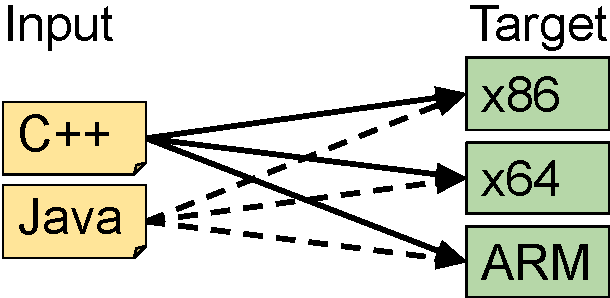
\includegraphics[width=0.8\textwidth]{figures/compilation_process_without_ir.pdf}
    %     \caption[short]{}
    %     \label{fig:compilation_process_no_ir}
    % \end{subfigure}\hfill%
    % This aligns the subfigures on one line.
    % \begin{subfigure}{0.55\textwidth}
        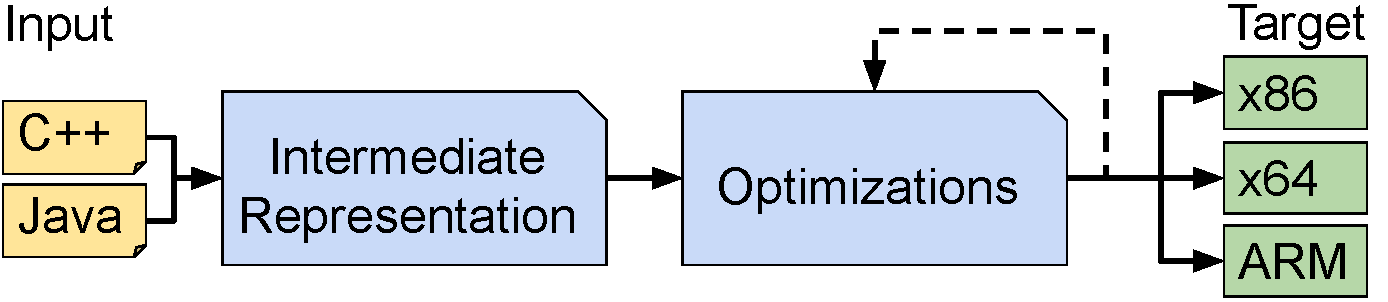
\includegraphics[width=\textwidth]{figures/compilation_process_with_ir.pdf}
        % \caption[short]{}
        % \label{fig:compilation_process_ir}
    % \end{subfigure}
    \caption{The job of a compiler: converting an input language (C++, Java) to machine code a specific architecture (x86, x64, ARM) can execute.  The dotted line denotes a self-loop the compiler employs for its various optimizations it runs.}
    \label{fig:compilation_process}
\end{figure*}

%=================================================================================
% Architectural Synthesis
%=================================================================================
\subsubsection{Architectural Synthesis}
\label{sec:synthesis}

Architectural synthesis is the automatic mapping of a high-level description to its corresponding low-level implementation.
It serves as an abstraction allowing the design and creation of complex architectures that might be untenable to create while simultaneously lowering the domain-specific knowledge a user must employ.
In traditional architectural synthesis, a designer writes a specification in a language like Verilog or VHDL\footnote{Very High Speed Integrated Circuit (VHSIC) Hardware Description Language (VHDL)} to describe how the device should operate.
The specification comes in the form of netlists --- each component has connections between itself and some set of other components.
This specification is then sent to a synthesis engine which attempts to place and route the components with their connections, as prescribed by the netlists.
Placement and routing is constrained by the specification (e.g., signal timing, space, or component size): two components must reside near enough to each other or the signal will not travel between the components within the specified clock-cycle, ruining the computation.
After the successful synthesis of the design the device is sent for fabrication.

In hardware design, architectural synthesis began with designers placing and routing discrete gates (components) by hand; placing an \textsf{XOR} or \textsf{NAND} gate and connecting their inputs and outputs by hand\jason{cite?}.
Shortly thereafter, designers created more complex components by combining groups of discrete gates into one larger, more complex component.
Thus, instead of placing a series of \textsf{NAND} gates, they would place a full-adder\footnote{a component capable of doing basic arithmetic.}.
This simple grouping quickly increased the complexity and capabilities of both the designers and their fabricated devices.
% This abstraction is, in principle, currently employed by hardware architects today.

In hardware architecture, the mapping between components and their low-level implementations are mature. In many hardware design architectures, component selection is straightforward and obvious --- an architect needs to add numbers, so they employ a full adder.
In the fluidic context this mapping isn't so clear; there are numerous constraints that require a priori knowledge that directly impacts the components that are selected for use during execution.
A case not present in the classical context of hardware architecture: a hardware architect need only know that arithmetic will occur, they require no other knowledge -- nothing about the types, size, or quantity of numbers. \jasoni{From Brian: I would specify something more like at the end of the day we only have to care if the electical value is high or low, and everything else is built on top of that single idea whereas with microfulidics the basics are much more complex. In architecture we would care about type (numerics) and size (bithwidth).}
For instance, the length of mixer (by time or by physical size) is dependent upon several properties pertaining to the input fluids, (e.g., viscosity). 
The 3D$\mu$F tool\cite{sanka20193d} has component generators which are capable of meeting architectural needs such as parameterizing the number outputs in a dilution bridge or the length and number of turns in a serpentine mixer. While this easies the burden of creating new components to meet architectural requirements, it still requires a large amount of domain expertise to know what parameters to specify to meet the fluidic needs. To the best of our knowledge there is only one previous work which utilizes user specified parameters describing the fluid properties and the desired dilution to generate a serpentine mixer which can meet those requirements \cite{grimmer2018meander}.


% \Cref{fig:synthesis_process} details the synthesis of a microfluidic device beginning with a high level specification written in \bs. The specification generates a netlist \cref{fig:net_list}, a hierarchical list of connections between components which apply operations to fluids.
% The netlist is generated by parsing the high-level \bs code into a directed acyclic graph (DAG) representing the flow of data through the program, which can be directly translated into the netlist.
% %and then converting the DAG directly into a netlist.
% Each node in the DAG is converted into a component which matches that functionality and the parameters supplied to it by the user (described below), while edges are translated as connections.
% From the netlist, the synthesis workflow aims to place all components on a chip \cref{fig:placement}.
% Once a valid placement is found, the synthesis tool attempts to route pathways between the components defined in the netlist \cref{fig:routing}.
% Assuming placement and routing succeed, the synthesis tool can fabricate the device \cref{fig:fabricated_chip}.

% \briani{consider if we want the above and below sections to be a single section on synthesis?}

%=================================================================================
% Component Generation & Selection
%=================================================================================
% \subsection{Component Generation \& Selection}
% \label{sec:component_selection}
% \tysoni{this section is difficult to read/follow... It seems you don't know what you're trying to say.  As this seems to be background info, state explicitly what has been done while delineating what is the new contribution}

% Continuous-flow microfluidic devices use the geometries of the device's design in order to utilize fluid dynamics to induce some type of desired fluidic outcome. 
% While there may be a direct translation from a function to a component for functions which only take fluidic parameters, components which have additional non-fluidic parameters are more difficult to translate.
% Coupling these non-fluidic parameters which are provided by the user with the fact that components are fixed after fabrication necessitates the ability to generate a component that meets these specific parameters. 
% In order to accomplish this task, we use a combination of pre-created components for non-parameterized functions along with component generators which can generate components to meet the specific parameters provided by the user.
% Since currently the vast majority of continuous-flow microfluidic devices are fully designed by hand, there has been little work in the automatic generation of components based on user specific parameters.
% To our knowledge,  

%=================================================================================
% Fabrication Methods
%=================================================================================
\subsubsection{Fabrication Methods}
\label{sec:fabrication_methods}

The fabrication of flow-based microfluidic devices is a rich research area, with many significant contributions borrowed from traditional computer architecture fabrication.
While this paper doesn't claim any contributions for techniques, we do present 
%this contribution is 
a complete synthesis workflow which is dependent upon existing fabrication techniques.

Flow-based microfluidic devices rely on fluid continuously flowing through networks of components and channels.
These channels and components are patterned onto one or more layers on the device.
Each patterned layer may be imprinted in either a rigid substrate (e.g., acrylic) \cite{el2006cells,hung2005continuous,pamme2007continuous} or a flexible polymer (e.g., \textit{polydimethylsiloxane (PDMS))}\cite{xia1998soft}.
To enclose the patterned layer(s), a rigid non-patterned material (e.g., glass) may be bonded to the topmost patterned layer, preventing contaminants or particulates from reaching internal layers and/or fluids and provide stability for flexible substrates.
To provide I/O access for fluids, small holes are either drilled (rigid material) or punched (flexible material) into the device.

Creating the patterned layer is dependent upon technology.\jason{this is vague...}
In general, there is an inverse relationship between the size of the feature and cost of the fabrication equipment required; however, most biological media (e.g., cells, organisms, etc.) are not suited for arbitrarily small features.
For fabricating rigid substrates, desktop CNC milling\cite{lashkaripour2019performance,lashkaripour2018desktop} is representative of a lower-cost, larger feature-size fabrication method; microfabrication through photolithography is representative of a relatively higher-cost, smaller feature-size fabrication method.
CNC milling cuts channels into polycabonate thermoplastic polymers through the use of a drill bit, whereas microfabrication etches patterns into glass using photolithography.
While a biologist can use any fabrication technique available to them, ensuring compatibility between material and the biological media influences both the material and fabrication technique used for generating a device.

Fabricating devices comprised of flexible materials are both more complex and more expensive than that of a rigid material\cite{xia1998soft}. The most common flexible material used in continuous-flow microfluidics, polydimethylsiloxane (PDMS), is ideal for its durability however, it suffers from being permeable to certain fluids and its fabrication for use as a microfluidic medium requires the construction of a physical rigid mold (as the final design's negative) and the precise mixture of reactants and curing process for success. The curing process requires exposure to air and/or heat to imprint into the mold before being attached to a rigid substrate to cap the stamped fluidic channel and component design. When working with small features, additional steps such as degassing to remove bubbles is also necessary, rending this as both costly and error-prone -- particularly when done by hand.

%production of a physical mold is required for photolithography. For flexible materials, such as PDMS, 
%it must first be in a liquid state so it can be poured onto the mold.
%The liquid then, once exposed to air and/or heat, partially harden to imprint the mold's pattern.
%Once the patterned medium has partially cured, it can then be mounted on a rigid substrate.
%However, this process is complicated by the necessity of additional steps such as degassing to remove bubbles; increasing time and cost of fabrication, and implicitly hindering scalability.

Another fabrication technique, Additive manufacturing (e.g., 3D printing\cite{gong2016high,rogers20153d,waheed20163d}) creates enclosed rigid 3D structures by %not placing any material where a channel should exist.
encapsulating the design within rigid material.
Additive manufacturing removes the need to bond distinct patterned layers; a key advantage over other fabrication techniques.
This advantage, however, comes with 2 costs: 3D printing is opaque, unlike glass or PDMS, which makes the use of fluid imaging almost impossible.
Second, recent research has shown that different 3D printing technologies introduce materials that expose different toxicity levels %and that these levels, in the most extreme cases, 
, though these can be remedied by exposure to ultraviolet light\cite{oskui2015assessing}.

Each of the existing fabrication methods have their strengths and weaknesses; however, they all share a common setback: the requirement of the manual placement of components and routing between them.
This bottleneck demonstrates a clear and present need for an automated tool that handles the synthesis of a device from a high-level language.

\begin{figure*}[htb]
    \centering
    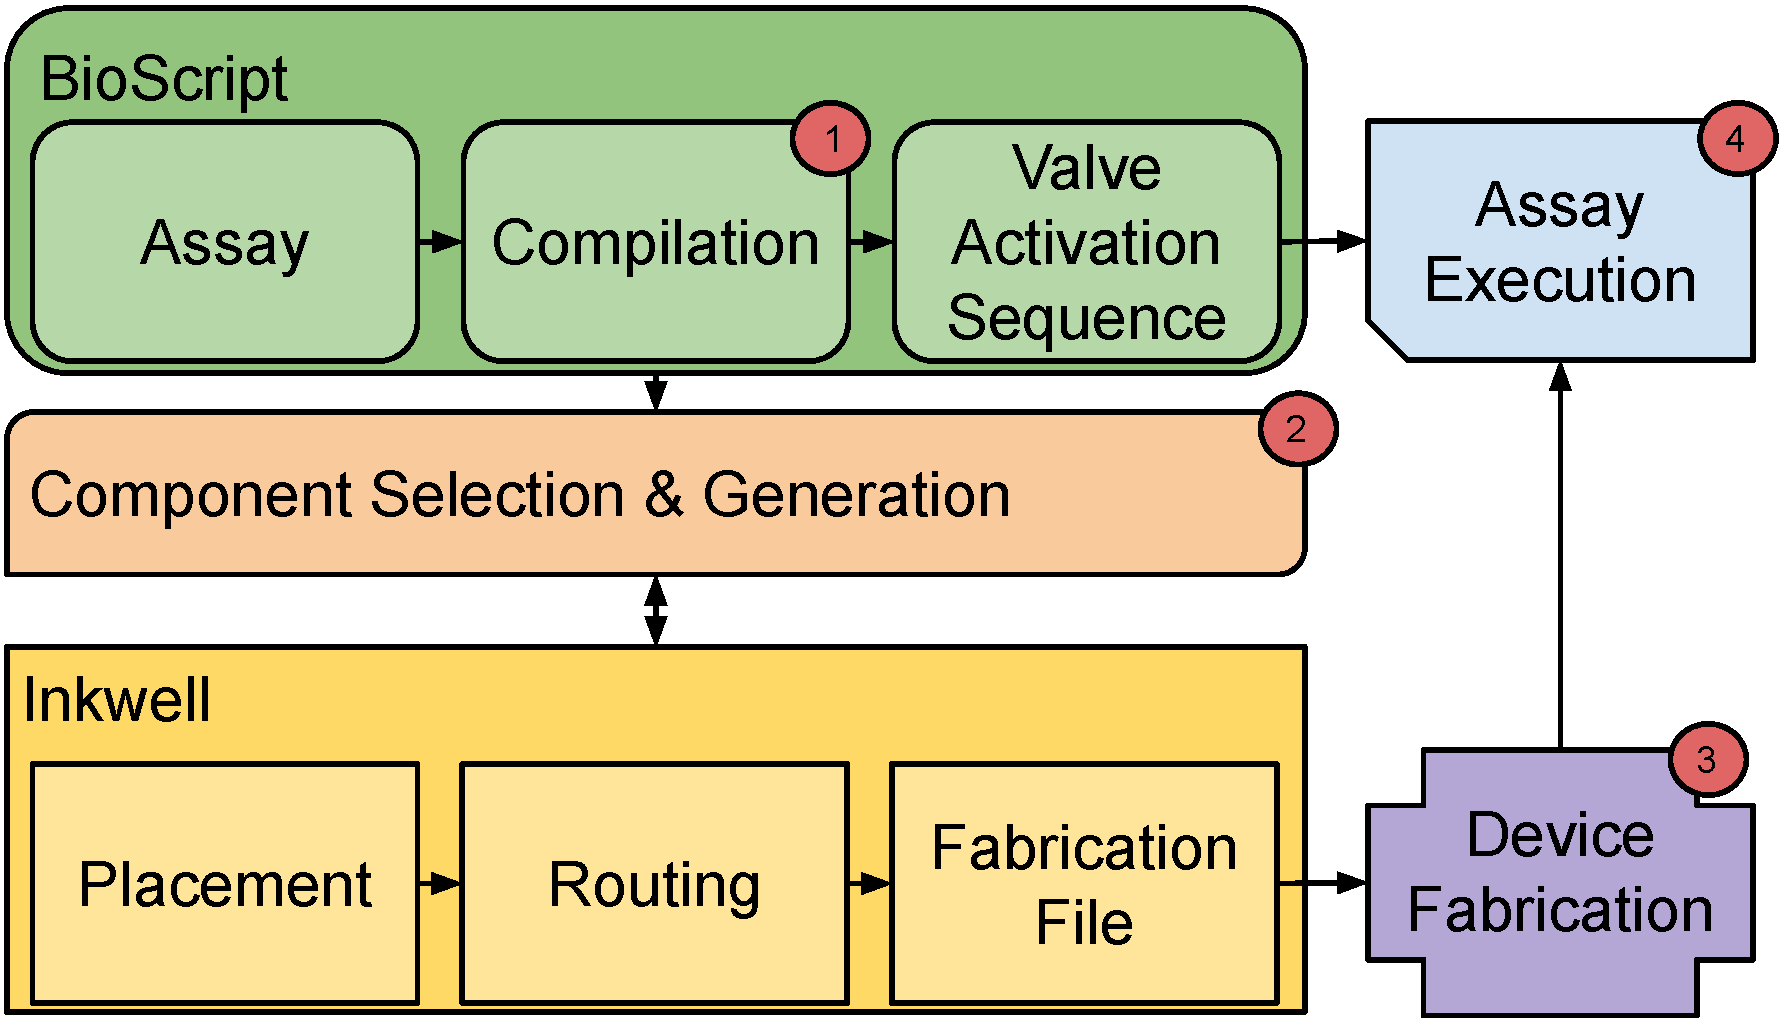
\includegraphics[width=0.8\textwidth]{figures/system_overview.pdf}
    \caption{Overview of the systems\protect{\cite{ott2018bioscript,mcdaniel2018design}} responsible for transforming an assay to the corresponding microfluidic device.}
    \label{fig:workflow}
\end{figure*}



\begin{figure*}[tb]
\centering
    \begin{subfigure}{0.35\textwidth}
        \begin{lstlisting}
manifest "hydrochloric acid"
manifest buffer

instructions:
hcl = dispense "hydrochloric acid"
buf = dispense buffer
dilution = mix hcl with buf
dispose buf
        \end{lstlisting}
        \caption[short]{}
        \label{fig:bs_program}
    \end{subfigure}
    %
    \begin{subfigure}{0.35\textwidth}
        \begin{lstlisting}
components: {
    input_1,
    input_2,
    mixer_1,
    output_1
},
netlist: {
    (input_1, mixer_1),
    (input_2, mixer_1),
    (mixer_1, output_1)
}
        \end{lstlisting}
        \caption[short]{}
        \label{fig:net_list}
    \end{subfigure}
    % Intentional blank line here.
    
    % End intentional blank line.
    \begin{subfigure}{0.33\textwidth}
        \fbox{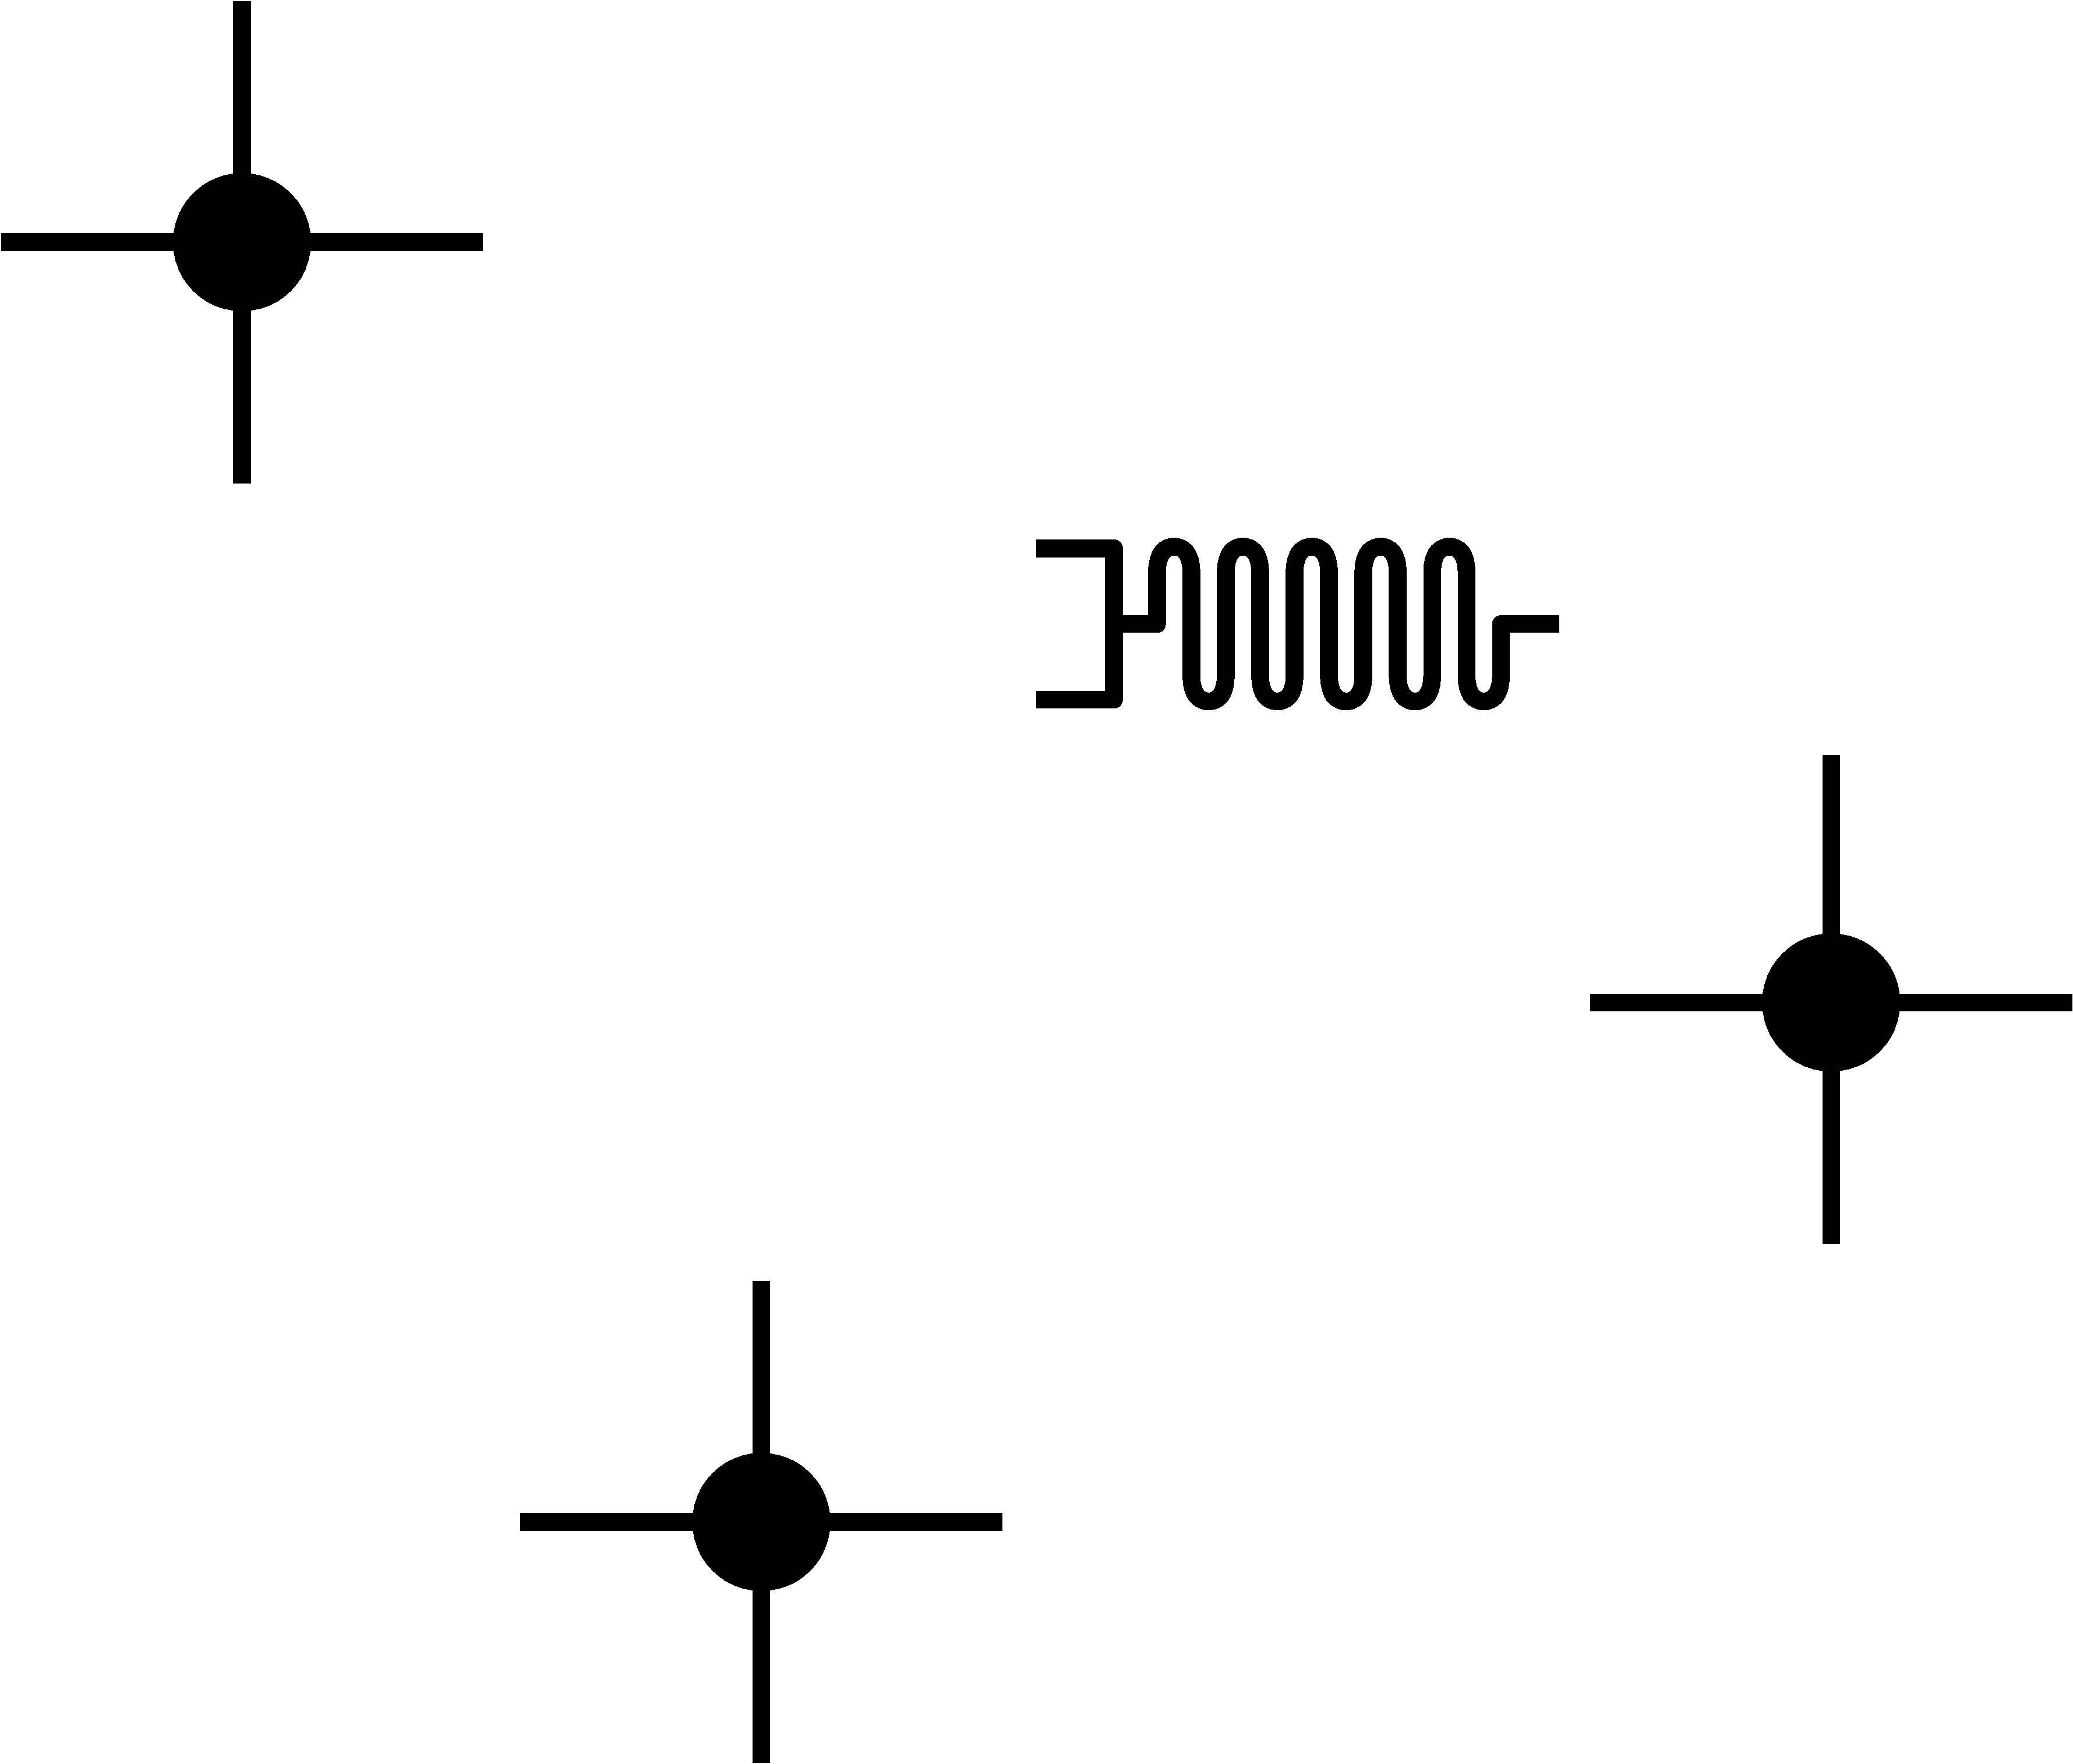
\includegraphics[width=0.9\textwidth]{figures/synthesis_process_placement.pdf}}
        \caption[short]{}
        \label{fig:placement}
    \end{subfigure}
    \begin{subfigure}{0.33\textwidth}
        \fbox{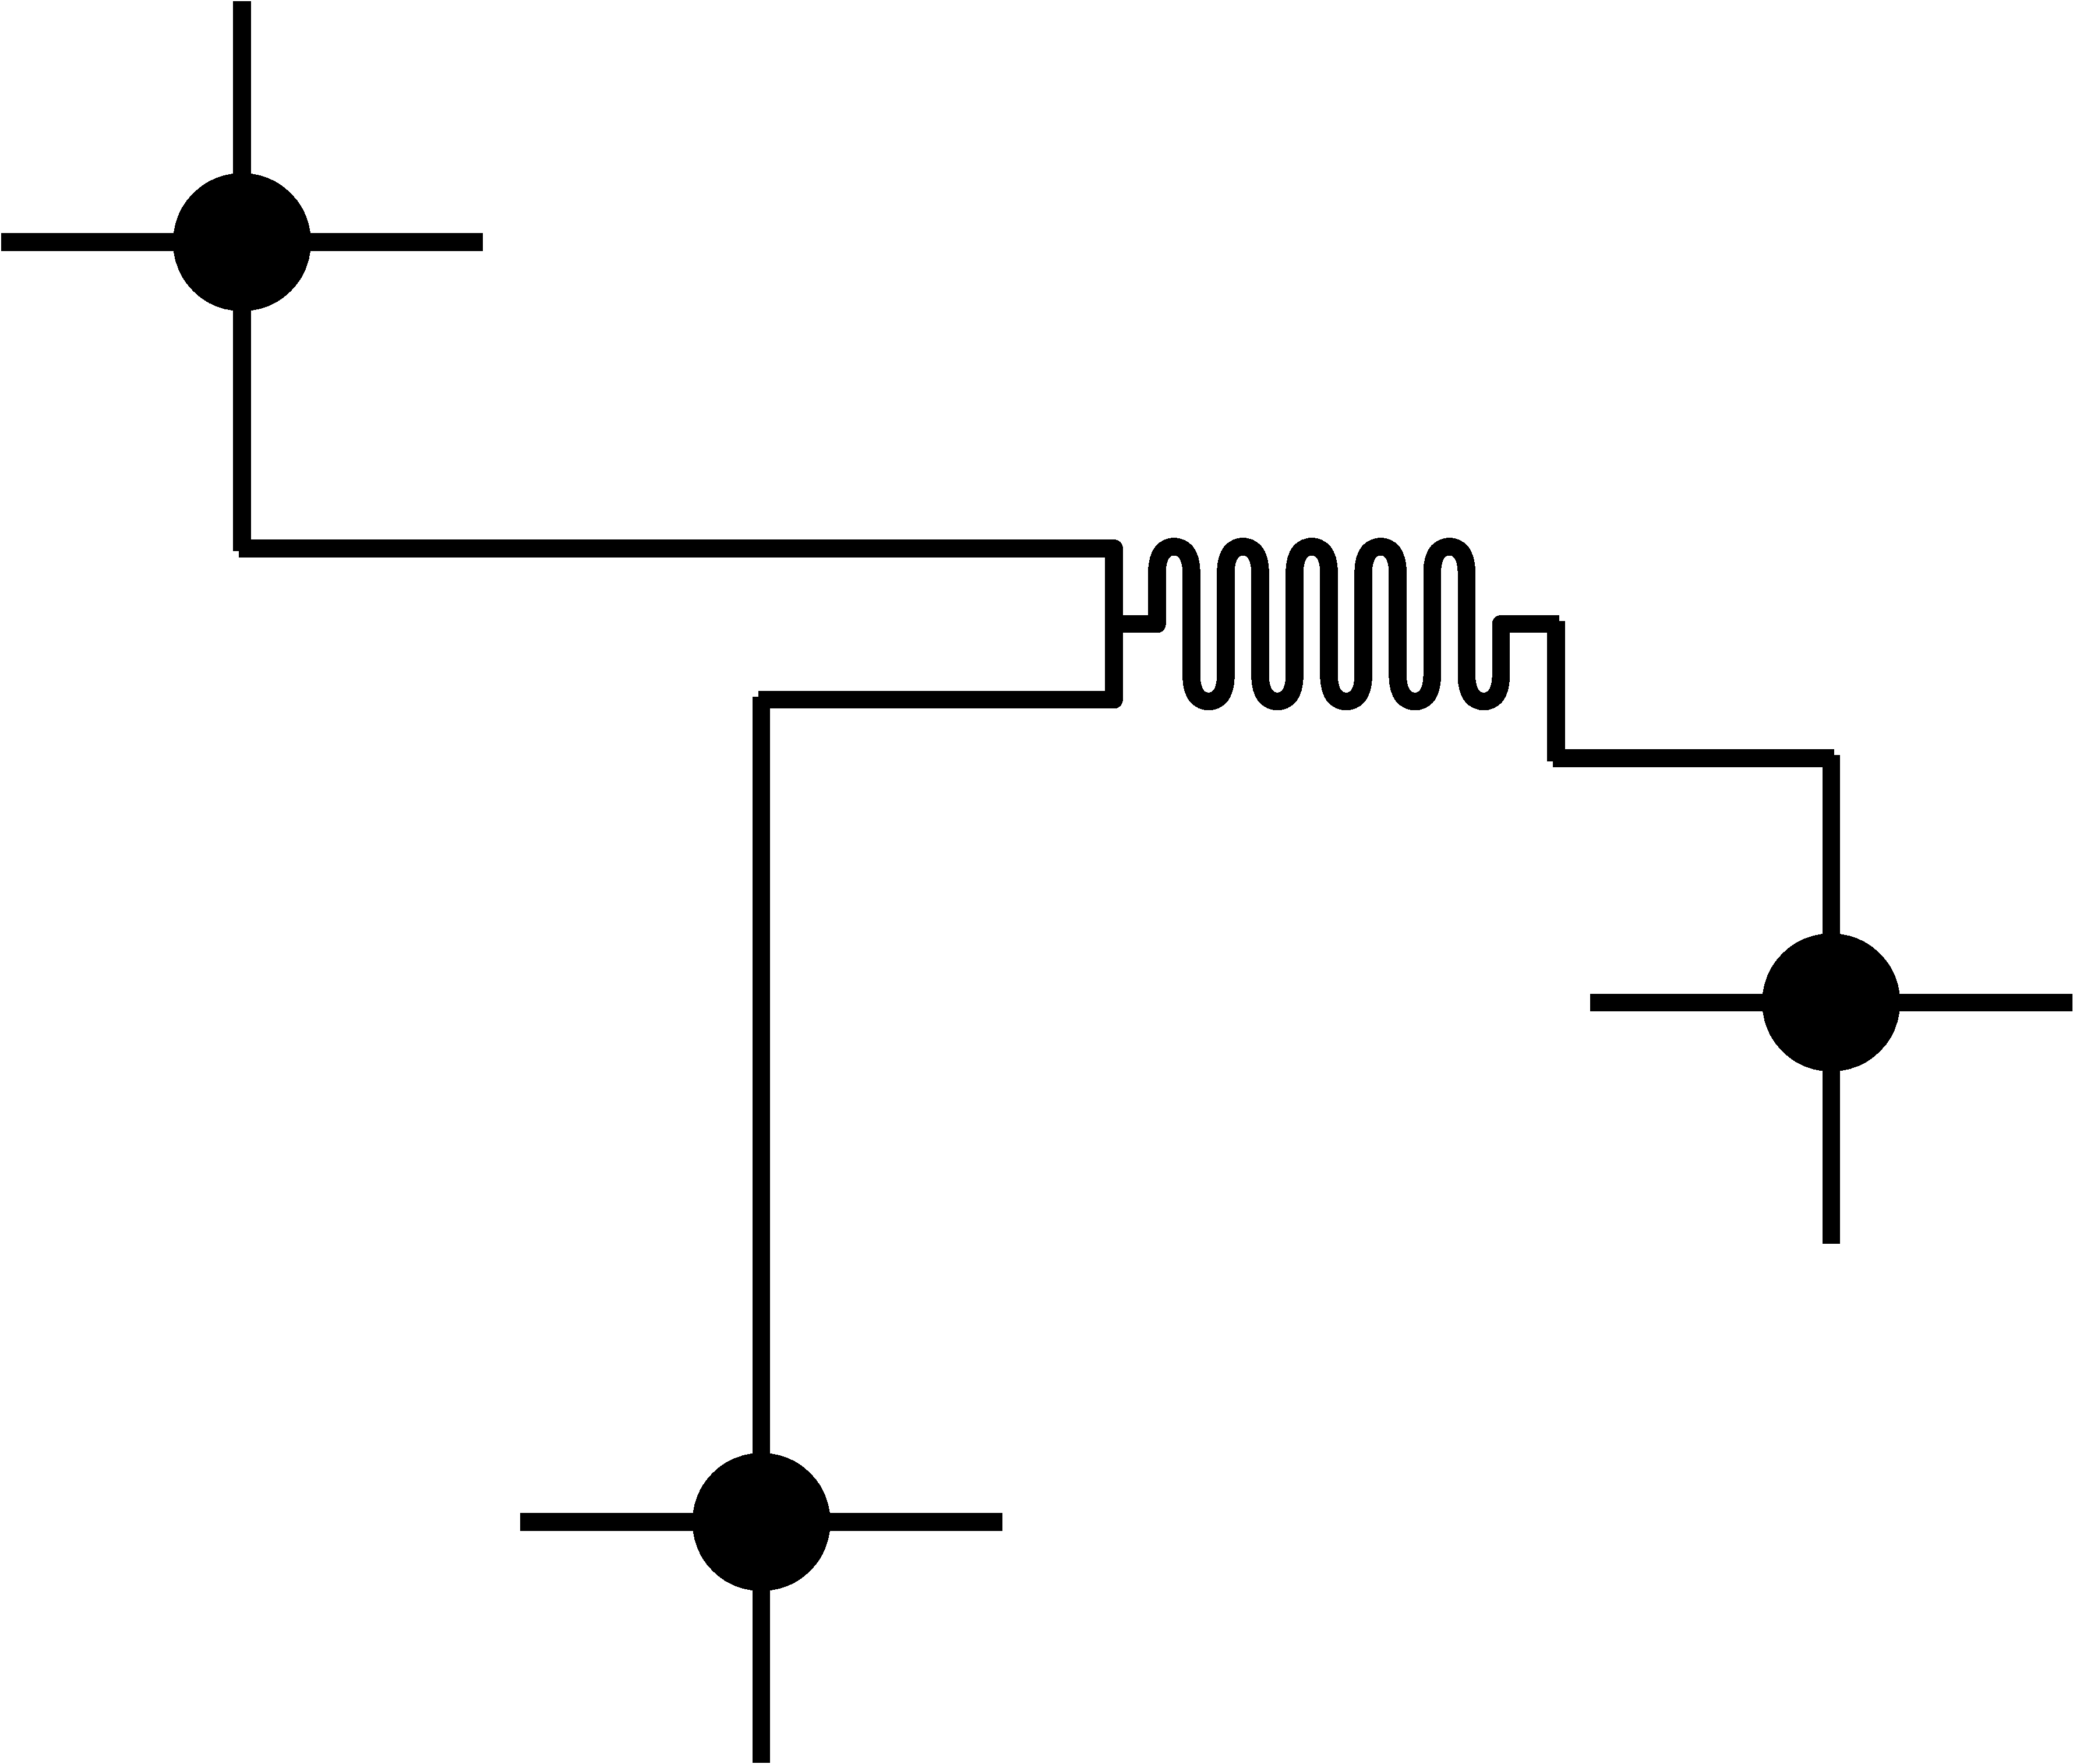
\includegraphics[width=0.9\textwidth]{figures/synthesis_process_routing.pdf}}
        \caption[short]{}
        \label{fig:routing}
    \end{subfigure}
    \begin{subfigure}{0.33\textwidth}
        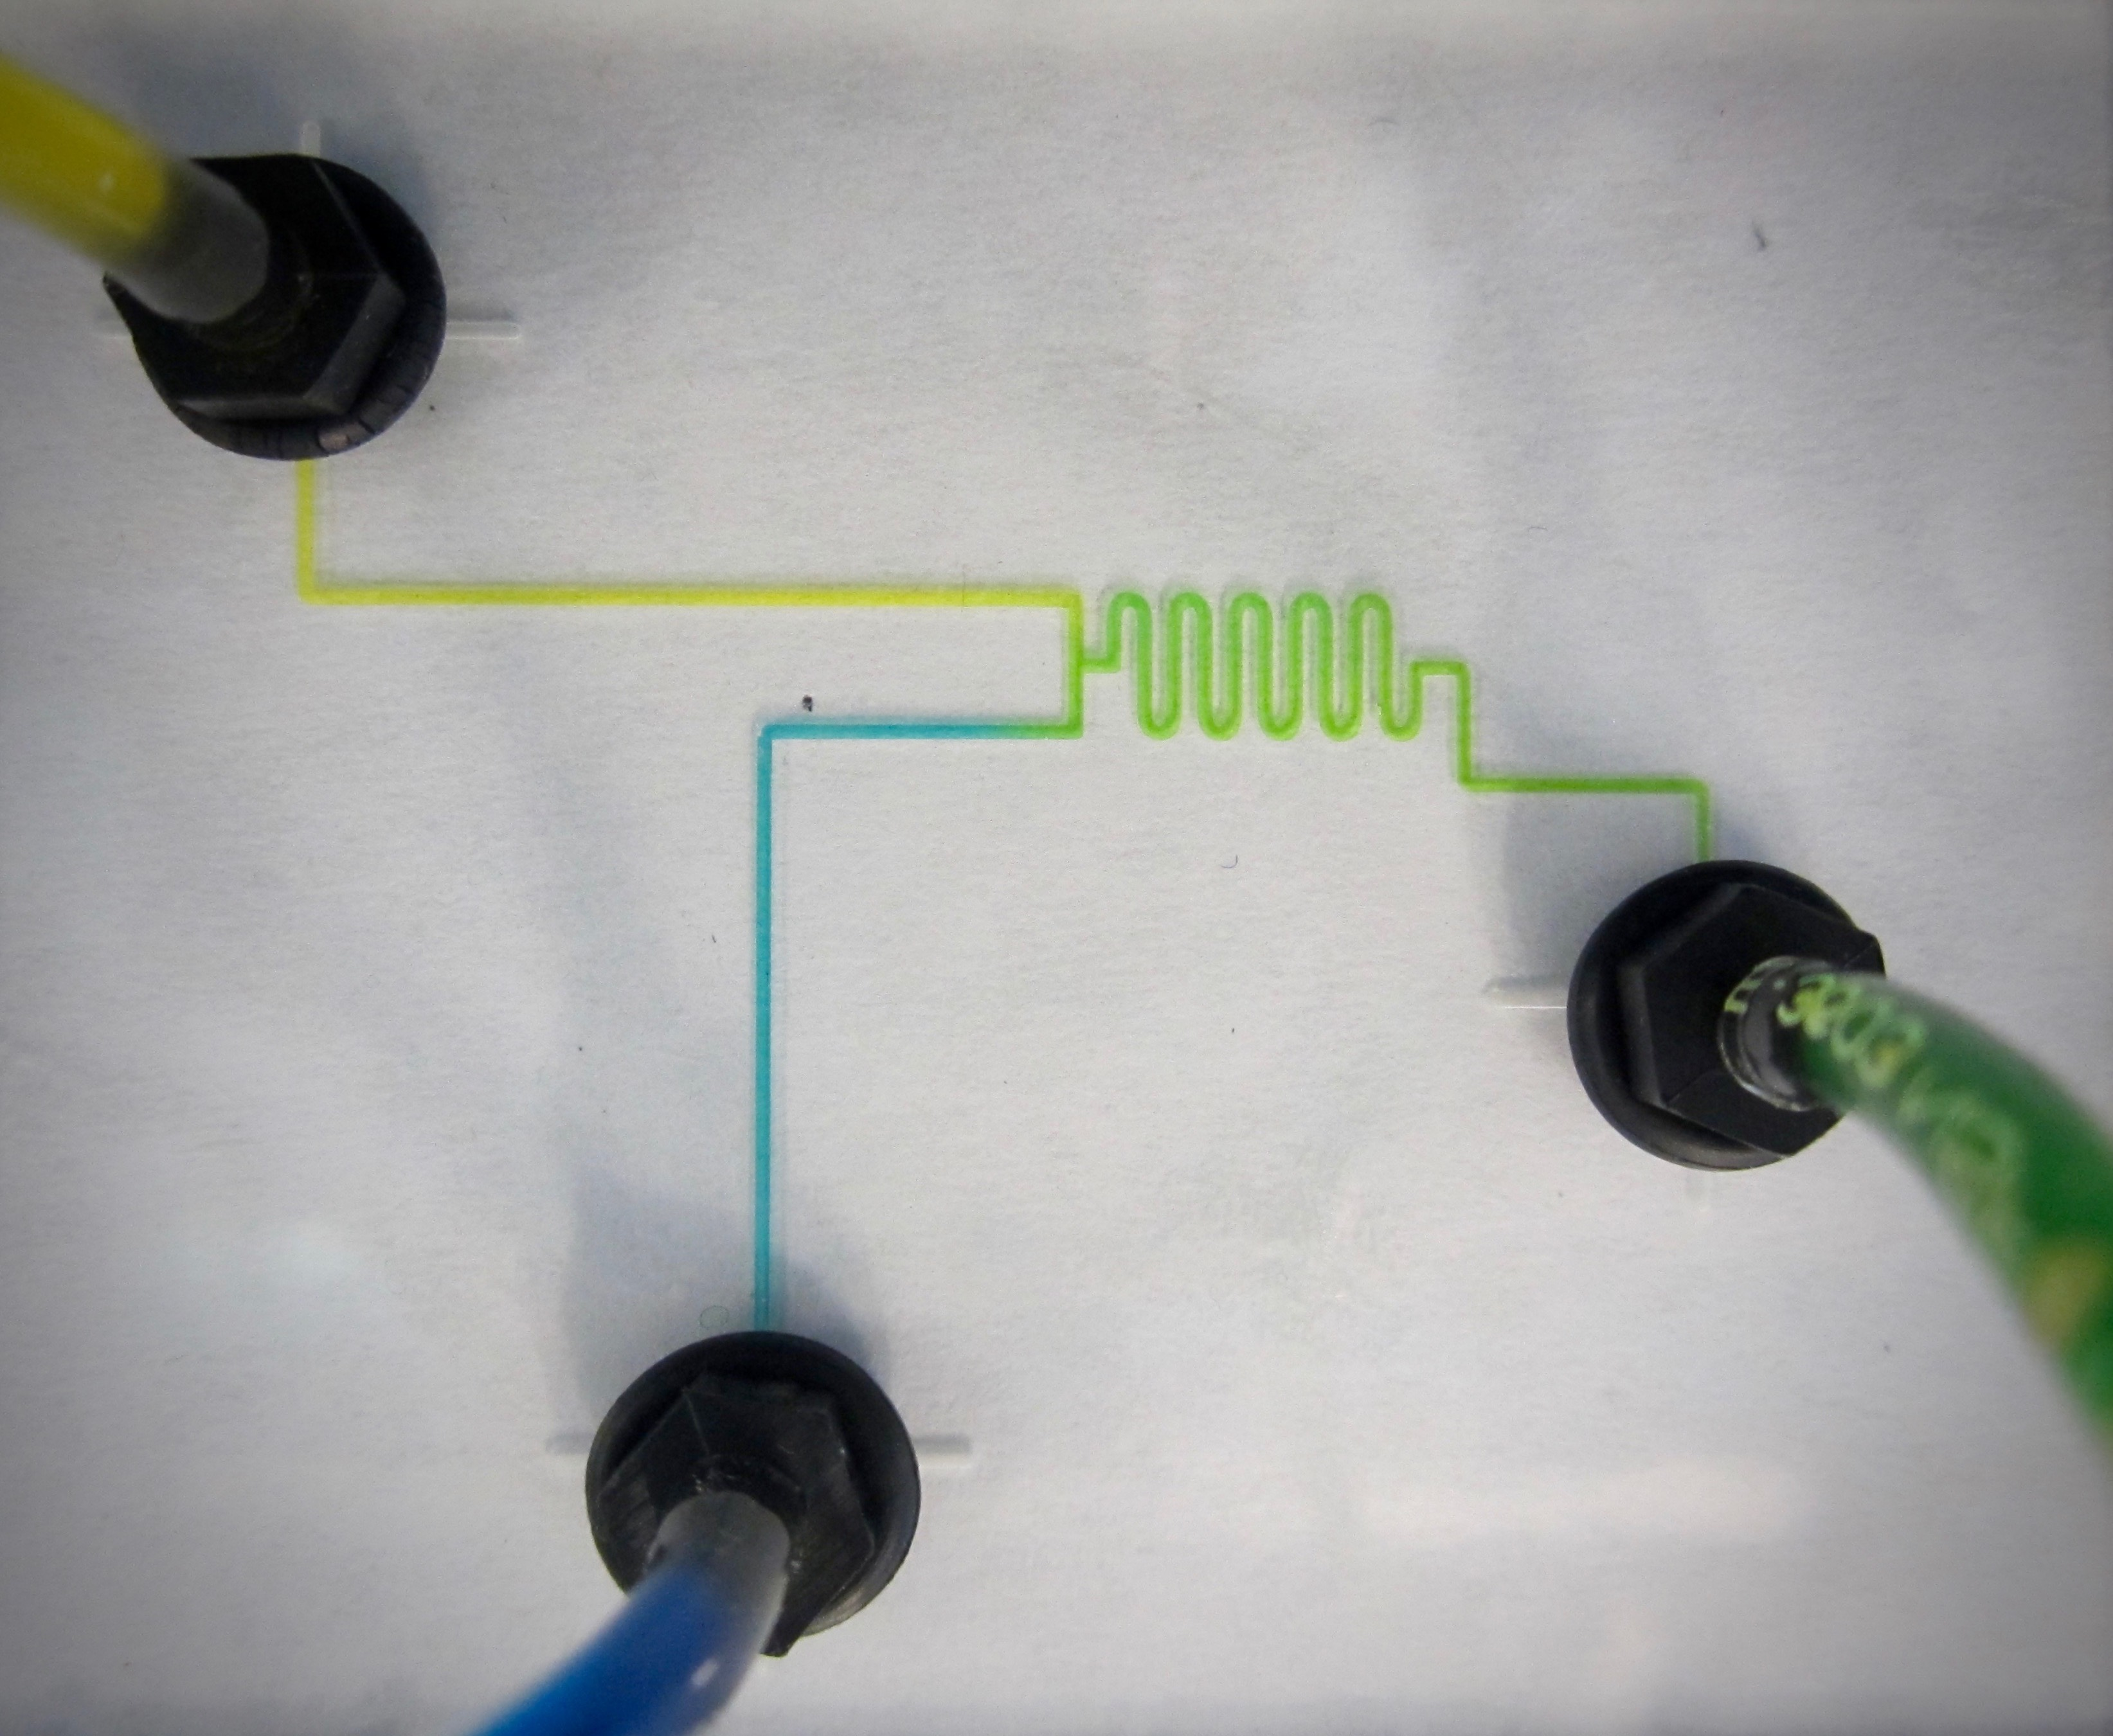
\includegraphics[width=0.97\textwidth]{figures/synthesized_mixer.jpg}
        \caption[short]{}
        \label{fig:fabricated_chip}
    \end{subfigure}
    \caption{Fabricating a flow-based devices begins with a \bs{} program (\cref{fig:bs_program}).  In \cref{fig:net_list} the \bs{} compiler then generates the components and connections (netlist).  A synthesis tool will then attempt to place the components on a device\Cref{fig:placement} and further attempts to route the connections prescribed in the netlist\cref{fig:routing}.  If both placement and routing are successful, the device can be fabricated (\cref{fig:fabricated_chip}) using any of the fabrication processes currently used.}
    \label{fig:synthesis_process}
\end{figure*}